\documentclass{article}

\usepackage[utf8]{inputenc}

%\usepackage{natbib}
\usepackage{hyperref}

\usepackage{graphicx}

\usepackage[colorinlistoftodos]{todonotes}

\usepackage{parskip}
\setlength{\parskip}{10pt} 

\usepackage{tikz}
\usetikzlibrary{arrows, decorations.markings}

\usepackage{outlines}

\usepackage{chngcntr}
\counterwithout{figure}{section}

\usepackage{pgfgantt}



\begin{document}


\begin{titlepage}
  

\centering
  
  
{\scshape\LARGE Master thesis Planning Report\\}
  
\vspace{0.5cm}
  
{\huge\bfseries Injection of Information to Embodied Agents\\}

  
\vspace{2cm}
  
{\Large Yasmeen Emampoor (gusemampya@student.gu.se)\\}
  
\vspace{1.0cm}
  
{\large Supervisor: Simon Dobnik (FLoV)\\}
  
\vspace{1.5cm}

\end{titlepage}
  
\section{Introduction}
\subsection{Background}
\todo{Why is it relevant?}

\subsection{Aim}
\todo{The aim is a brief description of the task and its intended outcome.}
The aim of this thesis is to identify ways in which prior or extra knowledge can be used to improve model performance in an EQA task. 

\subsection{Formulation}
\todo{The formulation of the problem at hand and the assignment. This should include an extended version of the scientific problem definition and references to knowledge within the area given in the thesis proposal.}

Hypotheses: 
\begin{outline}
	\1 The VQA model does consider the visual features when answering the questions.
		\2 If true, additional view points can improve performance in the VQA task. 
	\1 Additional semantic information can be used to improve performance in the VQA task. 
	\1 Additional semantic information can be used to improve performance in Navigation task. 
\end{outline}
 
\subsection{Limitations}
\todo{This chapter describes what issues will not be dealt with in the work.}
The main dataset of questions and answers available for EQA was automatically generated, and may contain some errors. One example of this is shown in Fig.~\ref{fig:err_ex}, in which a VQA model answered that the sofa in the living room is tan, but the ground truth answer is that it is yellow. However, looking at the image, I see a tan sofa and a yellow armchair. It seems that an error was likely made in the automatic question/answer generation, identifying the armchair as a sofa, but the model is not making the same error. \\
\begin{figure}[h]
	\centering
	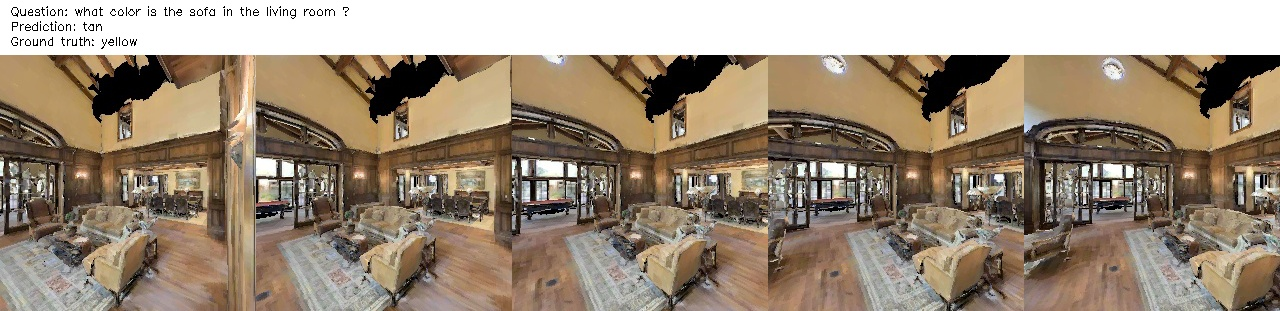
\includegraphics[width=\textwidth]{ckpt_0_121_image.jpg}
	\caption{Error Example}
	\label{fig:err_ex}
\end{figure}
Certain colors, such as brown, are also over represented in the dataset. However, I plan to work with this dataset as is, rather than attempting to balance presence of colors, or manually remove incorrect question answer pairs. This is both due to time limitations, and due to not wanting to introduce artificial balance--many things in houses are made of wood, and are therefore brown. It's not necessarily a bad thing for the system to expect tables to be brown, as long as it is also actually looking for a table to answer the question. \\
A dataset was collected using humans via Amazon Mechanical Turk, but it relies on a house dataset that is no longer available. \\
\todo{classification vs generation}
 

\section{Methodology}
\todo{The methodology chapter describes how the work is structured. It includes workflows, design of experiments and use of various data collection methods.}
\todo{mltgpu, metrics under consideration, blindfolded check after every change, enable the semantic sensor during VQA (talk about semantic annotations from matterport), implement look-around, enable the semantic sensor during navigation, discussion of other semantic options}

I am starting with the Embodied Question Answering baseline in Habitat-Lab, which consists of three parts, a CNN for initial feature extraction, a question answering module, and a navigation module, called Pacman\cite{embodiedqa}. I am using the EQA task dataset, which was created using code to automatically generate questions and answers to correspond with scenes in the Matterport3D dataset\cite{matterport}. \\

\section{Schedule}
\begin{ganttchart}[
	hgrid=true,
	vgrid=true
	]{1}{17}
	\gantttitle{Schedule}{17} \\
	\gantttitlelist{5, ..., 21}{1} \\
	\ganttbar{Getting GPU Access}{2}{2} \\
	\ganttbar{Attending related presentation}{2}{2} \\
	\ganttbar{Learning Habitat}{1}{6} \\
	\ganttbar{Writing Seminar I}{2}{2} \\
	\ganttbar{Train\&Eval.Baseline, blindfolded\&normal}{6}{7} \\
	\ganttlinkedbar{Enable Semantic Sensor during VQA}{7}{10} \\
	\ganttbar{Implement Look Around}{7}{10} \\
	\ganttbar{Enable Semantic Sensor during Nav}{11}{13} \\
	\ganttbar{Writing!}{14}{17} \\
	\ganttbar[bar/.append style={fill=red}]{GPU Off}{8}{8}
\end{ganttchart}

\todo{find date for Ali's presentation, add to chart}
\todo{make a gantt bar for uncertain tasks}


\section{Risk Analysis and Ethical Considerations}
\todo{running out of time, resource issues}
\todo{ethical concerns: where is this data coming from? Levels of abstraction that mask human input/biases.}


\bibliographystyle{ieeetr}
\bibliography{references}

\end{document}

